%!TEX encoding = IsoLatin

%
% Exemple de rapport
% par Pierre Tremblay, Universite Laval
% modifi� par Christian Gagne, Universite Laval
% 14/01/2011 - version 1.3
% modifi� par Robert Bergevin, Universit� Laval
% 24/11/2011
% modifi� par Jean-Yves Chouinard, Universit� Laval
% 11/01/2016
% modifi� par Jean-Yves Chouinard, Universit� Laval
% 04/01/2017
%

%
% Modele d'organisation d'un projet LaTeX 
% rapport/      dossier racine et fichier principal
% rapport/fig   fichiers des figures
% rapport/tex   autres fichiers .tex
%

% ** Preambule **
%
% Ajouter les options au besoin :
%    - "ULlof" pour inclure la liste des figures, requis si "\begin{figure}" utilise
%    - "ULlot" pour inclure la liste des tableaux, requis si "\begin{table}" utilise
%
\documentclass[12pt,ULlof,ULlot]{ULrapport}

% Chargement des packages supplementaires (si absent de la classe)
\usepackage[ansinew]{inputenc}
\usepackage[autolanguage]{numprint}
\usepackage{icomma}
%\usepackage[options]{nom_du_package}

% Definition d'une commande pour presenter des cellules multilignes dans un tableau
\newcommand{\cellulemultiligne}[1]{\begin{tabular}{@{}c@{}}#1\end{tabular}}

% Definition de colonnes en mode paragraphe avec alignement ajustable
% Cette definition requiert le chargement du package "array"
%    - alignement horizontal, parametre #1 : - \raggedright (aligne a gauche)
%                                            - \centering (centre)
%                                            - \raggedleft (aligne a droite)
%    - alignement vertical, parametre #2 : - p (aligne en haut)
%                                          - m (centre)
%                                          - b (aligne en bas)
%    - largeur, parametre #3 : longueur
\newcolumntype{Z}[3]{>{#1\hspace{0pt}\arraybackslash}#2{#3}}

% Definitions des parametres de la page titre
\TitreProjet{Titre du projet}                         % Titre du projet
\TitreRapport{Rapport de projet -- version 0}                       % Titre du rapport
\Destinataire{Robert Bergevin, Luc Lamontagne et Simon Thibault}         % Nom(s) du destinataire
\NumeroEquipe{99}                                     % Numero de l'equipe
\NomEquipe{Les Gaulois}                               % Nom de l'equipe
\TableauMembres{%                                     % Tableau des membres de l'equipe
   111\,111\,111  & Abraracourcix    & \\\hline        % matricule & nom & \\\hline
   222\,222\,222  & Bonemine         & \\\hline        % matricule & nom & \\\hline
   333\,333\,333  & Falbala          & \\\hline        % matricule & nom & \\\hline
   444\,444\,444  & I�losubmarine    & \\\hline        % matricule & nom & \\\hline
   555\,555\,555  & Ordralphab�tix   & \\\hline        % matricule & nom & \\\hline
   666\,666\,666  & Tragicomix       & \\\hline        % matricule & nom & \\\hline
}
\DateRemise{31 janvier 2019}                           % Date de remis


% Contenu de l'historique des versions
\HistoriqueVersions{%                        % version & date & description \\\hline
         & 17 janvier 2006 & cr�ation du document \\\hline
   1.0   & 22 janvier 2006 & illustration des capacit�s de \LaTeX: chapitre et sections, note en bas de page, r�f�rence dynamique, figure, insertion d'image, tableau, �quations, r�f�rences bibliographiques, liste\\\hline
   1.1   & 14 janvier 2007 & refonte compl�te: introduction de la classe, page titre, exemples \LaTeX, unit�s SI et r�gles d'�criture, recommandations typographiques\\\hline
   1.2   & 6 d�cembre 2007 & r�organisation des chapitres, ajout de l'historique des versions, ajouts des options ULlof et ULlot, ajout d'exemples de tableaux, corrections mineures\\\hline
   1.3   & 14 janvier 2011 & reformatage de l'exemple, changements � l'organisation des figures\\\hline
   1.3.1 & 24 novembre 2011 & matricules � 9 chiffres, titre du rapport\\\hline
   1.4   & 11 janvier 2016 & mise � jour pour la session d'hiver 2016\\\hline
	 1.4.1 &  4 janvier 2017 & mise � jour pour la session d'hiver 2017\\\hline
}


% Corps du document

\begin{document}

%   Chapitres
%!TEX encoding = IsoLatin

\chapter{Introduction}
\label{s:intro}

� faire



%!TEX encoding = IsoLatin

%
% Chapitre "Structure d'un rapport technique"
%

\chapter{Rapport technique}
\label{s:structure_rapport}

Un \emph{rapport technique} est un document dont la structure interne joue un r�le de premier plan. En effet, d�s les premiers instants de la lecture, le lecteur comprendra rapidement la structure adopt�e et �laborera des rep�res mentaux qui lui faciliteront grandement la t�che lorsqu'il consultera le rapport afin d'y retrouver l'information qu'il recherche. Il est donc tout aussi essentiel d'y fournir l'information technique, que de la regrouper et de la hi�rarchiser selon une approche logique, coh�rente et consistante tout au long de l'ouvrage.


\section{Structure}

Un rapport technique est globalement constitu� de trois parties majeures: les \emph{pages liminaires}, le \emph{corps} et les \emph{parties annexes}.


\subsection{Pages liminaires}

Les pages liminaires (\og front matter \fg) regroupent les pages plac�es au d�but de l'ouvrage, en pr�c�dant le corps. Elles contiennent les �l�ments suivants:
\begin{itemize}
   \item la page de titre (obligatoire);
   \item l'historique des versions (obligatoire);
   \item les remerciements (facultatif);
   \item la table des mati�res (obligatoire);
   \item la liste des figures (obligatoire si le rapport contient des figures);
   \item la liste des tableaux (obligatoire si le rapport contient des tableaux).
\end{itemize}
Les pages de cette premi�re partie sont num�rot�es en chiffres romains.


\subsection{Corps}

Le corps, ou le texte (\og main matter \fg), est l'essence m�me de l'un ouvrage. La seconde partie constitue donc le c\oe ur du document, il s'agit des diff�rents chapitres requis pour couvrir l'ensemble du sujet pr�sent�. La num�rotation des pages y est faite en chiffres arabes, en repartant de la page 1, et ce jusqu'� la fin du document. Le premier chapitre introduit le travail. Il permet, d'une part, d'en expliquer le contexte et, d'autre part, il d�finit le contenu du travail.


\subsection{Parties annexes}

Les parties  (\og back matter \fg) d'un ouvrage comprennent g�n�ralement:
\begin{itemize}
   \item la bibliographie\footnote{Il est � noter que bien que l'usage g�n�ral permette de diff�rencier la bibliographie, qui contient un ensemble de r�f�rences reli�es � l'ouvrage, de la liste des ouvrages cit�s, il est habituel, pour un rapport technique, de ne retrouver que la liste des ouvrages cit�s dans le texte, sous la d�nomination \og Bibliographie \fg.} (obligatoire);
   \item les annexes (facultatives);
      \begin{itemize}
         \item la liste des sigles et acronymes (obligatoire);
         \item le glossaire (facultatif);
         \item le lexique (facultatif);
         \item tout d�tail (calculs, mesures, etc.) qui alourdirait inutilement le corps de l'ouvrage;
      \end{itemize}
   \item l'index (facultatif).
\end{itemize}
Ces derni�res composantes contiennent le mat�riel dont la pr�sentation est compl�mentaire � l'ouvrage, mais dont la pr�sence n'est pas requise � l'int�rieur de la seconde partie.


\section{Recommandations face � la r�daction}

Cette section regroupe diff�rents conseils permettant d'am�liorer la qualit� globale du rapport technique.


\subsection{Usage de la classe \texttt{ULrapport}}

La classe \texttt{ULrapport} g�n�re automatiquement la page de titre, l'historique des versions et la table des mati�res. Il est � noter que la liste des figures n'est ajout�e que si l'option \og \texttt{ULlof} \fg\ est sp�cifi�e dans la commande d�clarant la classe de document (soit la commande \og \verb|\documentclass[]{ULrapport}| \fg). De m�me, la liste des tableaux n'appara�t que si l'option \og \texttt{ULlot} \fg\ est sp�cifi�e. Chacune de ces listes est requise d�s que les objets flottants correspondants sont utilis�s.

L'auteur est responsable d'ajouter le corps de l'ouvrage et les annexes appropri�es.


\subsection{Utilisation judicieuse des figures}

Le bouquin de \bsc{Parker} et \bsc{Th�rien} traite en d�tail la probl�matique de l'utilisation des �l�ments visuels, tels que photographies, illustrations, graphiques et diagrammes~\cite[ch. 4]{PAR91}. Il est important de bien doser la complexit� des �l�ments graphiques du rapport par une hi�rarchisation des informations et un choix du niveau de d�tail. Voici en r�sum� quelques recommandations afin d'optimiser l'impact des figures dans un rapport technique:
\begin{itemize}
   \item assurez la lisibilit�;
   \item �vitez la surcharge;
   \item pr�f�rez les dessins vectoriels aux images binaires;
   \item �vitez les croquis faits � main lev�e;
   \item assurez que tout texte apparaissant dans une figure soit r�dig� en fran�ais;
   \item lorsqu'une figure est extraite d'un autre document, fournissez la r�f�rence appropri�e dans la l�gende;
   \item lorsqu'une figure est extraite d'un document r�dig� en anglais, traduisez sa l�gende.
\end{itemize}

Il est finalement recommand� d'user de figures avec discernement. Autant une figure appropri�e sert efficacement � appuyer le propos, autant l'usage d'images inutiles, telles les logos de compagnie et les photographies g�n�riques de composants usuels, n'apporte rien d'utile. Le lecteur peut m�me y interpr�ter une volont� d'effectuer du remplissage.


\subsection{Emploi de tableaux pertinents}

Les tableaux permettent de pr�senter l'information d'une fa�on ordonn�e et concise. Chaque ligne et chaque colonne d'un tableau doivent �tre clairement identifi�es, respectivement, dans la premi�re colonne et dans la premi�re ligne. Lorsque des valeurs chiffr�es sont rapport�es, il importe d'en indiquer les unit�s SI.

L'�num�ration de sp�cifications techniques � l'int�rieur de paragraphes ou m�me de listes est tout d'abord inefficace du point de vue de l'espace requis. D'autre part, la lecture de telles descriptions est aride, peu int�ressante et ne permet pas au lecteur de s'y r�f�rer ais�ment. Les tableaux se pr�tent beaucoup mieux � un tel usage. Il est ensuite tr�s simple de s'y r�f�rer et d'y retrouver une information pr�cise.





%!TEX encoding = IsoLatin

%
% Chapitre "Recommandations typographiques"
%

\chapter{Recommandations typographiques}
\label{s:typo}

Ce bref chapitre d�crit quelques r�gles typographiques de base applicables aux textes r�dig�s en fran�ais ou en anglais. Elles sont d�crites aux tableaux \ref{t:recommandations_typographiques} et \ref{t:recommandations_typographiques_legende}.
\begin{table}[htp]
   \footnotesize
   \centering
   \caption{Recommandations typographiques propres aux langues fran�aise et anglaise. L'ast�risque d�note celles qui sont prises en compte automatiquement par le package \texttt{babel}.}
   \label{t:recommandations_typographiques}
   \begin{tabular}{|l|l|c|c|l|c|c|}
      \hline\hline
      \multicolumn{1}{|c|}{}
      & \multicolumn{3}{c|}{\emph{fran�ais}}
      & \multicolumn{3}{c|}{\emph{anglais}}
      \\\cline{2-7}
      \multicolumn{1}{|c|}{\raisebox{1.4ex}[0ex][0ex]{\emph{�l�ment}}}
         % la commande "\raisebox" peut etre evitee en utilisant le package "multirow"
      & \multicolumn{1}{c|}{\emph{nom}}
      & \emph{signe}
      & \emph{code}
      & \multicolumn{1}{c|}{\emph{nom}}
      & \emph{signe}
      & \emph{code}
      \\\hline

      guillemets$^\ast$
      & doubles chevrons & \og\ldots\fg & \verb|\og \fg|
      & double quotes    & ``\ldots''   & \verb|`` ''|
      \\

      liste � puces$^\ast$
      & tiret moyen      & --           & \verb|--|
      & bullet           & $\bullet$    & \verb|$\bullet$|
      \\

      abr�viation
      & c'est-�-dire     & c.-�-d.      &
      & \emph{id est}    & \emph{i.e.}  &
      \\

      abr�viation
      & par exemple              & p.\ ex.      &
      & \emph{exempli gracia}    & \emph{e.g.}  &
      \\

      abr�viation
      & pages            & p.      &
      & pages            & pp.     &
      \\

      \hline\hline
   \end{tabular}
\end{table}

\begin{table}[htp]
   \footnotesize
   \centering
   \caption{Recommandations propres aux langues fran�aise et anglaise quant � l'emplacement des l�gendes. Notez que ces r�gles ne sont pas prises en compte par le package \texttt{babel}.}
   \label{t:recommandations_typographiques_legende}
   \begin{tabular}{|l|l|l|}
      \hline\hline
      \multicolumn{1}{|c|}{\emph{objet flottant}}
      & \multicolumn{1}{c|}{\emph{fran�ais}}
      & \multicolumn{1}{c|}{\emph{anglais}}
      \\\hline

      figure
      & apr�s l'objet graphique
      & apr�s l'objet graphique
      \\

      table
      & avant la grille
      & apr�s la grille
      \\

      \hline\hline
   \end{tabular}
\end{table}

Toute figure et tout tableau doit �tre r�f�renc� dans le texte du rapport par son num�ro (p. ex. \og figure~\ref{f:exemple_figure_pdf} \fg\  ou \og tableau~\ref{t:prix_materiaux} \fg). Dans un rapport r�dig� en anglais, contrairement � un rapport en fran�ais, la majuscule est toujours utilis�e (p. ex. \og Figure~\ref{f:exemple_figure_pdf} \fg\  ou \og Table~\ref{t:prix_materiaux} \fg).

%!TEX encoding = IsoLatin

%
% Chapitre "Exemples LaTeX"
%

\chapter{Exemples \LaTeX}
\label{s:exemples_LaTeX}

Le pr�sent chapitre est plus sp�cifiquement utilis� pour illustrer les capacit�s de \LaTeX\ � l'aide de divers exemples. On y traite, entre autres, de plusieurs d�tails concernant les objets flottants que sont les figures et les tableaux.


\section{Outils de r�f�rences}
\label{s:ref}

L'ouvrage de \bsc{Knuth}~\cite{KNU84} renferme une mine de renseignements sur le fonctionnement de \TeX. La premi�re r�f�rence introduisant \LaTeX\ est �videmment le bouquin de \bsc{Lamport} lui-m�me~\cite{LAM94}. Finalement \emph{The LaTeX Companion}~\cite{MIT04} constitue un excellent ouvrage g�n�ral d�crivant exhaustivement une s�lection des \og packages \fg\ disponibles les plus utiles, de m�me qu'une foule de d�tails permettant de modeler \LaTeX\ � sa guise.


\section{Exemples d'objets flottants}
\label{s:ex_obj_flottants}

Deux types d'objets flottants existent � l'int�rieur de \LaTeX: les figures et les tableaux. Dans chaque cas, il est essentiel de discerner l'objet fixe repr�sentant l'image ou la grille de l'objet flottant, la figure ou le tableau, respectivement. Chaque objet flottant comporte nominalement un objet fixe, ainsi qu'une l�gende.


\subsection{Exemples de figures}
\label{s:ex_figures}

\subsubsection{Objet graphique vectoriel de type PDF}
\label{s:ex_fig_PDF}

La figure~\ref{f:exemple_figure_pdf} fournit un exemple de figure utilisant un fichier vectoriel de type PDF d'\textsc{Adobe}. L'environnement \texttt{figure} y est employ�.
\begin{figure}[htp]
   \centering
   
\includegraphics[width=0.6\textwidth]{ul_logo}
   \caption{Exemple de figure faite � partir d'un fichier PDF d'\textsc{Adobe}. Logo de l'Universit� Laval.}
   \label{f:exemple_figure_pdf}
\end{figure}

Les commandes \verb|\centering|, \verb|\includegraphics|, \verb|\caption| et \verb|\label| sont aussi d�montr�es dans cette figure.

Il est important de noter que la l�gende, introduite par la commande \verb|\caption|, doit �tre plac�e apr�s l'�l�ment graphique (voir aussi le tableau~\ref{t:recommandations_typographiques_legende} � la page~\pageref{t:recommandations_typographiques_legende}).


\subsubsection{Objets graphiques binaires de type JPEG}
\label{s:ex_fig_JPEG}

La figure~\ref{f:exemple_figure_jpeg} (montr�e � la page~\pageref{f:exemple_figure_jpeg}) fournit un exemple de figure utilisant un fichier binaire de type JPEG. Le m�me environnement et les m�mes commandes qu'� la section pr�c�dente sont employ�es.
\begin{figure}[htp]
   \centering
   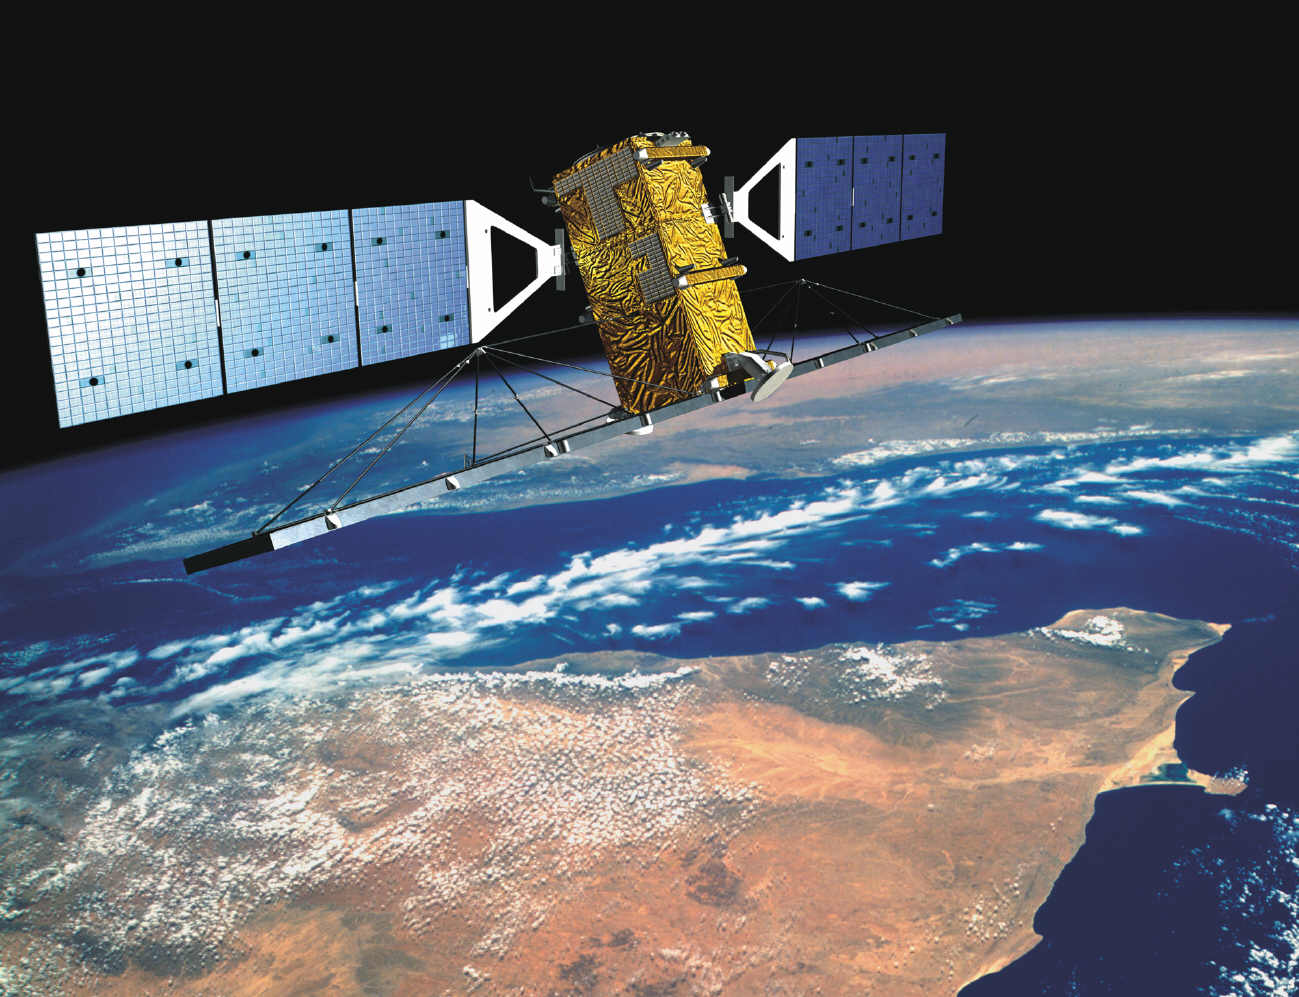
\includegraphics[width=\textwidth]{radarsat}
   \caption{Exemple d'une figure con�ue � partir d'un fichier JPEG. Repr�sentation artistique du satellite canadien RADARSAT-2.}
   \label{f:exemple_figure_jpeg}
\end{figure}


\subsection{Exemples de tableaux}
\label{s:ex_tableaux}

\subsubsection{Tableau simple}
\label{s:ex_tableau_simple}

Le tableau~\ref{t:prix_materiaux} illustre l'utilisation de l'environnement \texttt{table}. Une grille r�alis�e � l'aide de l'environnement \texttt{tabular} constitue le c\oe ur de ce tableau.

\begin{table}[htp]
   \centering
   \caption{Exemple de tableau. Liste de prix des mat�riaux de r�f�rence au 1 f�vrier 2006, telle que fournie par les Laboratoires des mines et des sciences min�rales.}
   \label{t:prix_materiaux}
   \begin{tabular}{|l|c|r|}
      \hline\hline
      \multicolumn{1}{|c|}{\emph{description}}
      & \emph{unit�}
      & \multicolumn{1}{c|}{\emph{prix}}
      \\ \hline
      Minerai d'uranium          & 100 g     & 95,00  \$  \\
      Minerai d'or               & 200 g     & 180,00  \$  \\
      Alliages de zinc-aluminium & 7 disques & 1500,00 \$  \\
      \hline\hline
   \end{tabular}
\end{table}

Les commandes \verb|\hline| et \verb|\multicolumn| sont aussi d�montr�es dans ce tableau.

Il est important de noter que la l�gende, introduite par la commande \verb|\caption|, doit �tre plac�e avant la grille (voir aussi le tableau~\ref{t:recommandations_typographiques_legende} � la page~\pageref{t:recommandations_typographiques_legende}).


\subsubsection{Tableau avec cellules multilignes}
\label{s:ex_tableau_simple2}

Le tableau~\ref{t:exemple_table} est un exemple o� certains �l�ments de la premi�re rang�e occupent plus d'une ligne de texte et doivent �tre centr�s verticalement.

\begin{table}[htp]
   \centering
   \caption{Exemple de tableau avec cellules multilignes. Illustration de l'usage de la commande \texttt{\textbackslash cellulemultiligne}. Statistiques de contacts satellite-station terrestre pour une p�riode de 10~jours.}
   \label{t:exemple_table}
   \begin{tabular}{|c|c|c|c|c|c|}
      \hline\hline
      \cellulemultiligne{\emph{station} \\ \emph{terrestre}}
      & \cellulemultiligne{\emph{nombre} \\ \emph{total de} \\ \emph{contacts}}
      & \cellulemultiligne{\emph{dur�e} \\ \emph{totale des} \\ \emph{contacts}}
      & \cellulemultiligne{\emph{nombre} \\ \emph{moyen de}
                           \\ \emph{contacts} \\ \emph{par jour}}
      & \cellulemultiligne{\emph{dur�e} \\ \emph{moyenne} \\ \emph{des} \\ \emph{contacts}}
      & \cellulemultiligne{\emph{dur�e} \\ \emph{moyenne}
                           \\ \emph{de contact} \\ \emph{par jour}}
      \\\hline
      A  & 18  &  64 min    & 1,8  & 3,56 min  &  6,4 min  \\
      B  & 17  &  56,2 min  & 1,7  & 3,31 min  &  5,6 min  \\
      C  & 34  & 119 min    & 3,4  & 3,49 min  & 11,9 min  \\
      D  & 16  &  51,1 min  & 1,6  & 3,19 min  &  5,1 min  \\
      \hline\hline
   \end{tabular}
\end{table}

Un autre environnement \texttt{tabular} y est utilis� pour chacune des cellules multilignes. La nouvelle commande \verb|\cellulemultiligne|, d�finie dans le pr�ambule, y est d'ailleurs employ�e explicitement afin de simplifier la r�daction.


\subsubsection{Tableau avec cellules contenant un long texte}
\label{s:ex_tableau_simple3}

Le tableau~\ref{t:exemple_table_texte} d�montre l'utilisation d'environnements de type paragraphe � l'int�rieur de cellules.

\begin{table}[htp]
   \centering
   \caption{Exemple de tableau avec cellules contenant des paragraphes. Illustration de l'usage de \texttt{\textbackslash Z}.}
   \label{t:exemple_table_texte}
   \begin{tabular}{|Z{\raggedright}{b}{4cm}|Z{\centering}{m}{4cm}|Z{\raggedleft}{p}{4cm}|}
      \hline\hline
      Exemple de texte un peu long, mais typographi� sans probl�me
         avec positionnement vertical r�f�r� en bas!
      & Exemple de texte un peu long, mais typographi� sans probl�me
         avec positionnement vertical centr�!
      & Exemple de texte un peu long, mais typographi� sans probl�me
         avec positionnement vertical r�f�r� en haut!
      \\
      \hline\hline
   \end{tabular}
\end{table}

La nouvelle d�finition de colonne \verb|\Z|, introduite dans le pr�ambule, y est d'ailleurs employ�e explicitement afin de simplifier la r�daction. Elle permet de pr�senter un long texte en d�finissant sa pr�sentation horizontale (gauche, centre ou droite), sa position verticale de r�f�rence (haut, centre, bas) et sa largeur.


\subsection{Autres tableaux possibles}
\label{s:autres_tableaux}

\subsubsection{Tableaux plus larges que le corps du texte}

Si vous d�sirez faire un tableau plus large, il y a moyen de le faire en utilisant la page en paysage (\og landscape \fg), utilisez alors l'environnement \texttt{sidewaystable} (fourni avec le package \texttt{rotating}). L'exemple qui suit montre comment s'y prendre.
\begin{verbatim}
\begin{sidewaystable}
   \centering
   \caption{L�gende du tableau.}
   \label{t:etiquette_de_tableau}
   \begin{tabular}{...}
      ...
   \end{tabular}
\end{sidewaystable}"
\end{verbatim}

L'environnement \texttt{sidewaysfigure} existe aussi pour les figures plus larges.


\subsubsection{Tableaux plus longs qu'une page}

Le package \texttt{longtable} fournit l'environnement \texttt{longtable} qui permet de typographier des tableaux qui parcourent plus d'une page. L'exemple qui suit montre comment s'y prendre.
\begin{verbatim}
\begin{longtable}{cc}
      \caption{L�gende du tableau.}
      \label{t:etiquette_de_tableau}         \\ \hline
      \emph{colonne 1} & \emph{colonne 2}    \\ \hline
   \endfirsthead
      \caption[]{(suite)}                    \\ \hline
      \emph{colonne 1} & \emph{colonne 2}    \\ \hline
   \endhead
      \hline \multicolumn{2}{r}{\emph{Suite � la page suivante}}
   \endfoot
      \hline
   \endlastfoot
   ... & ... \\
   ... & ... \\
\end{longtable}
\end{verbatim}
Il est � noter que, contrairement aux tableaux standard requ�rant \texttt{table} et \texttt{tabular}, un tableau complet (objet flottant et grille, voir \S\ref{s:ex_tableaux}) est r�alis� avec l'environnement \texttt{longtable}. Par d�faut ce tableau est centr� horizontalement, ce qui peut �tre ais�ment chang� par le biais d'un argument optionnel (\texttt{[l]} ou \texttt{[r]}). Un exemple de l'utilisation de ce type de tableau est fourni au tableau~\ref{t:longtable_example}.


\begin{longtable}{lcc}
      \caption{Les 100~premiers �l�ments du tableau p�riodique class�s par ordre alphab�tique.}
      \label{t:longtable_example}
      \\ \hline
      \multicolumn{1}{c}{%
         \cellulemultiligne{\emph{nom de} \\ \emph{l'�l�ment} \\ \emph{chimique}}}
      & \emph{symbole}
      & \cellulemultiligne{\emph{nombre} \\ \emph{atomique}}
      \\ \hline
   \endfirsthead
      \caption[]{(suite)}
      \\ \hline
      \multicolumn{1}{c}{%
         \cellulemultiligne{\emph{nom de} \\ \emph{l'�l�ment} \\ \emph{chimique}}}
      & \emph{symbole}
      & \cellulemultiligne{\emph{nombre} \\ \emph{atomique}}
      \\ \hline
   \endhead
      \hline \multicolumn{3}{r}{\emph{Suite � la page suivante}}
   \endfoot
      \hline
   \endlastfoot
   actinium       & Ac  & 89  \\
   aluminum       & Al  & 13  \\
   am�ricium      & Am  & 95  \\
   antimoine      & Sb  & 51  \\
   argent         & Ag  & 47  \\
   argon          & Ar  & 18  \\
   arsenic        & As  & 33  \\
   astate         & At  & 85  \\
   azote          & N   & 7   \\
   baryum         & Ba  & 56  \\
   berk�lium      & Bk  & 97  \\
   b�ryllium      & Be  & 4   \\
   bismuth        & Bi  & 83  \\
%   Bohrium        & Bh  & 107 \\
   bore           & B   & 5   \\
   brome          & Br  & 35  \\
   cadmium        & Cd  & 48  \\
   calcium        & Ca  & 20  \\
   californium    & Cf  & 98  \\
   carbone        & C   & 6   \\
   c�rium         & Ce  & 58  \\
   c�sium         & Cs  & 55  \\
   chlore         & Cl  & 17  \\
   chrome         & Cr  & 24  \\
   cobalt         & Co  & 27  \\
   cuivre         & Cu  & 29  \\
   curium         & Cm  & 96  \\
%   Darmstadtium   & Ds  & 110 \\
%   Dubnium        & Db  & 105 \\
   dysprosium     & Dy  & 66  \\
   einsteinium    & Es  & 99  \\
   erbium         & Er  & 68  \\
   �tain          & Sn  & 50  \\
   europium       & Eu  & 63  \\
   fer            & Fe  & 26  \\
   fermium        & Fm  & 100 \\
   fluor          & F   & 9   \\
   francium       & Fr  & 87  \\
   gadolinium     & Gd  & 64  \\
   gallium        & Ga  & 31  \\
   germanium      & Ge  & 32  \\
   hafnium        & Hf  & 72  \\
%   Hassium        & Hs  & 108 \\
   h�lium         & He  & 2   \\
   holmium        & Ho  & 67  \\
   hydrog�ne      & H   & 1   \\
   indium         & In  & 49  \\
   iode           & I   & 53  \\
   iridium        & Ir  & 77  \\
   krypton        & Kr  & 36  \\
   lanthane       & La  & 57  \\
   lawrencium     & Lr  & 103 \\
   lithium        & Li  & 3   \\
   lut�cium       & Lu  & 71  \\
   magn�sium      & Mg  & 12  \\
   mangan�se      & Mn  & 25  \\
%   Meitnerium     & Mt  & 109 \\
%   mend�l�vium    & Md  & 101 \\
   mercure        & Hg  & 80  \\
   molybd�ne      & Mo  & 42  \\
   n�odyme        & Nd  & 60  \\
   n�on           & Ne  & 10  \\
   neptunium      & Np  & 93  \\
   nickel         & Ni  & 28  \\
   niobium        & Nb  & 41  \\
%   nob�lium       & No  & 102 \\
   osmium         & Os  & 76  \\
   or             & Au  & 79  \\
   oxyg�ne        & O   & 8   \\
   palladium      & Pd  & 46  \\
   phosphore      & P   & 15  \\
   platine        & Pt  & 78  \\
   plomb          & Pb  & 82  \\
   plutonium      & Pu  & 94  \\
   polonium       & Po  & 84  \\
   potassium      & K   & 19  \\
   pras�odyme     & Pr  & 59  \\
   prom�thium     & Pm  & 61  \\
   protactinium   & Pa  & 91  \\
   radium         & Ra  & 88  \\
   radon          & Rn  & 86  \\
   rh�nium        & Re  & 75  \\
   rhodium        & Rh  & 45  \\
   rubidium       & Rb  & 37  \\
   ruth�nium      & Ru  & 44  \\
%   Rutherfordium  & Rf  & 104 \\
   samarium       & Sm  & 62  \\
   scandium       & Sc  & 21  \\
%   Seaborgium     & Sg  & 106 \\
   s�l�nium       & Se  & 34  \\
   silicium       & Si  & 14  \\
   sodium         & Na  & 11  \\
   soufre         & S   & 16  \\
   strontium      & Sr  & 38  \\
   tantale        & Ta  & 73  \\
   techn�tium     & Tc  & 43  \\
   tellure        & Te  & 52  \\
   terbium        & Tb  & 65  \\
   thallium       & Tl  & 81  \\
   thorium        & Th  & 90  \\
   thulium        & Tm  & 69  \\
   titane         & Ti  & 22  \\
   tungst�ne      & W   & 74  \\
%   Ununbium       & Uub & 112 \\
%   Ununhexium     & Uuh & 116 \\
%   Ununoctium     & Uuo & 118 \\
%   Ununpentium    & Uup & 115 \\
%   Ununquadium    & Uuq & 114 \\
%   Ununseptium    & Uus & 117 \\
%   Ununtrium      & Uut & 113 \\
%   Ununium        & Uuu & 111 \\
   uranium        & U   & 92  \\
   vanadium       & V   & 23  \\
   x�non          & Xe  & 54  \\
   ytterbium      & Yb  & 70  \\
   yttrium        & Y   & 39  \\
   zinc           & Zn  & 30  \\
   zirconium      & Zr  & 40  \\
\end{longtable}

Les diff�rentes sections permettent de sp�cifier le haut du tableau � la premi�re page (avant \verb|\endfirsthead|), puis le haut du tableau aux pages subs�quentes (avant \verb|\endhead|). De m�me il faut aussi indiquer le bas du tableau � sa derni�re page (avant \verb|\endlastfoot|), ainsi qu'aux pages pr�c�dentes (avant \verb|\endfoot|).

Il est tout � fait proscrit d'utiliser \texttt{longtable} pour des tableaux qui peuvent �tre pr�sent�s sur une seule page. En effet, il serait inopportun de scinder un tel tableau en deux parties.


\section{Ouvrages cit�s et URL}

Puisque Internet fournit maintenant de nombreux documents de r�f�rence, il importe de pouvoir citer les sites web correctement afin de permettre au lecteur d'y r�f�rer. Des r�gles d'�criture de telles r�f�rences bibliographiques sont d�crites sur le site de la biblioth�que~\cite{BIB07}. En particulier, ce dernier site sugg�re d'utiliser le format suivant pour r�f�rer correctement � un site web:
\begin{flushleft}\ttfamily
Auteur (Organisme ou auteur personnel dans le cas d'une page personnelle). \emph{Titre de la page d'accueil}, [Type de support]. Adresse URL: fournir l'adresse URL de la ressource (date de la consultation par l'usager: jour, mois, ann�e)
\end{flushleft}
La r�f�rence~\cite{BIB07} du pr�sent document en est un excellent exemple.







%!TEX encoding = IsoLatin

%
% Chapitre "Unit�s SI et r�gles d'�criture"
%

\chapter{Unit�s SI et r�gles d'�criture}
\label{s:SI}

La sp�cification de chaque quantit� physique implique l'usage de valeurs num�riques et d'unit�s. Ce chapitre en pr�sente les r�gles d'�criture qui ont fait l'objet d'accords internationaux. Les unit�s accept�es et les pr�fixes pouvant leur �tre juxtapos�s, ainsi que les r�gles r�gissant leur �criture, sont pr�sent�es en premier. Suivent ensuite les r�gles d'�criture des valeurs num�riques, de m�me que les conventions permettant la sp�cification d'incertitudes de mesure.

Il est important de pr�ciser que le strict respect des r�gles d'�criture du SI est n�cessairement de mise pour un rapport technique.


\section{Unit�s accept�es}
\label{s:unite_acceptees}

Cette section pr�sente les diff�rentes unit�s du Syst�me international d'unit�s (SI). Ces derni�res ont fait l'objet d'accords internationaux standardisant leur nom et leur symbole. Il s'ensuit que ces recommandations doivent �tre suivies � la lettre afin d'�viter toute interpr�tation fautive. Le SI se compose d'unit�s de base (\S\ref{s:unite_base}), d'unit�s d�riv�es (\S\ref{s:unite_derivees}) et enfin d'un certain nombre d'autres unit�s suppl�mentaires dont l'usage est reconnu (\S\ref{s:autres_unites}).


\subsection{Unit�s SI de base}
\label{s:unite_base}

Les 7~unit�s SI de base sont pr�sent�es au tableau~\ref{t:exemple_table_unites_base_SI}~\cite{BIP98}. Les noms adopt�s en fran�ais et en anglais sont fournis, les symboles sont toutefois les m�mes dans ces deux langues.

\begin{table}
   \centering
   \caption{Unit�s SI de base.}
   \label{t:exemple_table_unites_base_SI}
   \begin{tabular}{|Z{\raggedright}{m}{5cm}|c|c|l|}
      \hline\hline
      \multicolumn{1}{|c|}{\emph{grandeur de base}}
         & \multicolumn{1}{c|}{\emph{nom / name}}
         & \emph{symbole}
         & \multicolumn{1}{c|}{\emph{d�finition}}
         \\\hline
      longueur                     & m�tre / meter          & m    & 17\ieme{} CGPM, 1983  \\
      masse                        & kilogramme / kilogram  & kg   &  3\ieme{} CGPM, 1901  \\
      temps                        & seconde / second       & s    & 13\ieme{} CGPM, 1967  \\
      courant �lectrique           & amp�re / ampere        & A    &  9\ieme{} CGPM, 1948  \\
      temp�rature thermodynamique  & kelvin / kelvin        & K    & 13\ieme{} CGPM, 1967  \\
      quantit� de mati�re          & mole / mole            & mol  & 14\ieme{} CGPM, 1971  \\
      intensit� lumineuse          & candela / candela      & cd   & 16\ieme{} CGPM, 1979  \\
      \hline\hline
   \end{tabular}
\end{table}


\subsection{Unit�s SI d�riv�es}
\label{s:unite_derivees}

Afin de repr�senter les diff�rentes grandeurs physiques rencontr�es dans notre environnement, diff�rentes unit�s ont �t� d�riv�es � partir des unit�s SI de base. Le tableau \ref{t:exemple_table_unites_derivees_SI} donne les unit�s SI d�riv�es et les grandeurs physiques correspondantes~\cite{BIP98,BIP00}. Le tableau fournit aussi les symboles standard adopt�s par accords internationaux, ainsi que leurs �quivalents en unit�s SI de base.

\begin{table}
   \centering
   \caption{Unit�s SI d�riv�es.}
   \label{t:exemple_table_unites_derivees_SI}
   \begin{tabular}{|Z{\raggedright}{m}{4.9cm}|l|c|>{$}l<{$}|}
      \hline\hline
      \multicolumn{1}{|c|}{\emph{grandeur d�riv�e}}
         & \multicolumn{1}{c|}{\emph{nom}}
         & \emph{symbole}
         & \multicolumn{1}{c|}{\emph{expression}}
         \\\hline
      activit� & becquerel & Bq & \text{s}^{-1}  \\
      quantit� d'�lectricit�, charge �lectrique & coulomb & C & \text{s} \cdot \text{A}  \\
      temp�rature Celsius & degr� Celsius & \textcelsius & \text{K}  \\
      capacit� �lectrique & farad & F & \text{m}^{-2} \cdot \text{kg}^{-1} \cdot \text{s}^{4} \cdot \text{A}^{2}  \\
      dose absorb�e, �nergie massique, kerma & gray & Gy & \text{m}^{2} \cdot \text{s}^{-2}  \\
      inductance & henry & H & \text{m}^{2} \cdot \text{kg} \cdot \text{s}^{-2} \cdot \text{A}^{-2}  \\
      fr�quence & hertz & Hz & \text{s}^{-1}  \\
      �nergie, travail, quantit� de chaleur & joule & J & \text{m}^{2} \cdot \text{kg} \cdot \text{s}^{-2}  \\
      activit� catalytique & katal & kat & \text{s}^{-1} \cdot \text{mol}  \\
      flux lumineux & lumen & lm & \text{cd}  \\
      �clairement lumineux & lux & lx & \text{m}^{-2} \cdot \text{cd}  \\
      force & newton & N & \text{m} \cdot \text{kg} \cdot \text{s}^{-2}  \\
      r�sistance �lectrique & ohm & \textohm & \text{m}^{2} \cdot \text{kg} \cdot \text{s}^{-3} \cdot \text{A}^{-2}  \\
      pression, contrainte & pascal & Pa & \text{m}^{-1} \cdot \text{kg} \cdot \text{s}^{-2}  \\
      angle plan & radian & rad & 1  \\
      conductance �lectrique & siemens & S & \text{m}^{-2} \cdot \text{kg}^{-1} \cdot \text{s}^{3} \cdot \text{A}^{2}  \\
      �quivalent de dose & sievert & Sv & \text{m}^{2} \cdot \text{s}^{-2}  \\
      angle solide & st�radian & sr & 1  \\
      induction magn�tique & tesla & T & \text{kg} \cdot \text{s}^{-2} \cdot \text{A}^{-1}  \\
      diff�rence de potentiel �lectrique, force �lectromotrice & volt & V & \text{m}^{2} \cdot \text{kg} \cdot \text{s}^{-3} \cdot \text{A}^{-1}  \\
      puissance, flux �nerg�tique & watt & W & \text{m}^{2} \cdot \text{kg} \cdot \text{s}^{-3}  \\
      flux d'induction magn�tique & weber & Wb & \text{m}^{2} \cdot \text{kg} \cdot \text{s}^{-2} \cdot \text{A}^{-1}  \\
      \hline\hline
   \end{tabular}
\end{table}

Les noms anglais des unit�s SI d�riv�es sont les m�mes qu'en fran�ais, � l'exception de \og degree Celsius \fg\ et de \og steradian \fg.


\subsection{Autres unit�s en usage}
\label{s:autres_unites}

Des unit�s suppl�mentaires, bien que ne faisant pas partie formellement du Syst�me international d'unit�s sont couramment en usage. Le tableau~\ref{t:exemple_table_unites_dehors_SI} en pr�sente la liste~\cite{BIP98}.

\begin{table}
   \centering
   \caption{Unit�s en dehors du SI, mais en usage avec le SI.}
   \label{t:exemple_table_unites_dehors_SI}
   \begin{tabular}{|l|c|c|>{$}l<{$}|}
      \hline\hline
      \multicolumn{1}{|c|}{\emph{grandeur}}
         & \multicolumn{1}{c|}{\emph{nom / name}}
         & \emph{symbole}
         & \multicolumn{1}{c|}{\emph{valeur}}
         \\\hline
      temps                  & minute              & min
                             & 1 \text{~min} = 60 \text{~s}
      \\
      temps                  & heure / hour        & h
                             & 1 \text{~h} = 3600 \text{~s}
      \\
      temps                  & jour / day          & d
                             & 1 \text{~d} = 86400 \text{~s}
      \\
      angle plan             & degr� / degree      & \degres
                             & 1 \text{\degres} = (\pi/180) \text{~rad}
      \\
      angle plan             & minute              & $^\prime$
                             & 1^\prime = (\pi/10800) \text{~rad}
      \\
      angle plan             & seconde / second    & $^{\prime\prime}$
                             & 1^{\prime\prime} = (\pi/648000) \text{~rad}
      \\
      volume                 & litre               & l, L
                             & 1 \text{~l} = 10^{-3} \text{~m}^{3}
      \\
      masse                  & tonne / metric ton  & t
                             & 1 \text{~t} = 10^{3} \text{~kg}
      \\
      grandeur logarithmique & neper               & Np
                             & 1 \text{~Np} = 1
      \\
      grandeur logarithmique & bel                 & B
                             & 1 \text{~B} = (1/2) \ln 10 \text{~Np}
      \\
      \hline\hline
   \end{tabular}
\end{table}

Malheureusement une certaine confusion persiste autour des unit�s employ�es en technologie de l'information, il en r�sulte qu'aucun accord global ne soit intervenu. Un certain accord semble en voie de se r�aliser concernant le bit (symbolis� par \og bit \fg), surtout d� au fait que le m�me mot et le m�me symbole puissent �tre utilis�s en fran�ais et en anglais\footnote{Notez qu'afin d'�viter la confusion entre \og bit \fg\ et \og byte \fg, l'usage du symbole \og b \fg\ n'est pas recommand�.}. Quant � l'octet (8~bits), bien qu'un accord semble moins �vident � ce moment, l'usage du symbole \og o \fg\  se r�pand en fran�ais et ne cr�e aucune confusion avec d'autres unit�s. La situation diff�re en anglais, car le symbole \og B \fg\ est actuellement le plus r�pandu pour signifier \og byte \fg, malgr� la possible confusion avec le bel (voir tableau~\ref{t:exemple_table_unites_dehors_SI}).


\section{Pr�fixes recommand�s}

Le tableau~\ref{t:exemple_table_prefixes_SI} pr�sente l'ensemble des pr�fixes recommand�s actuellement en vigueur dans le Syst�me international d'unit�s, de m�me que les symboles correspondants \cite{BIP98}. Les pr�fixes choisis repr�sentent des puissances de 10. Bien qu'il existe des pr�fixes pour toutes les puissances de 10 incluses entre $10^{-3}$ et $10^{3}$, inclusivement, les autres pr�fixes ne correspondent qu'aux puissances de 10 qui sont multiples de 3 et qui sont comprises entre $10^{-24}$ et $10^{24}$.

\begin{table}
   \centering
   \caption{Pr�fixes et symboles du Syst�me international d'unit�s (SI). Les pr�fixes anglais sont les m�mes que les fran�ais, en leur retirant toutefois les accents.}
   \label{t:exemple_table_prefixes_SI}
   \begin{tabular}{|>{$}c<{$}|l|c|l|}
      \hline\hline
      \multicolumn{1}{|c|}{\emph{facteur}}
         & \multicolumn{1}{c|}{\emph{pr�fixe}}
         & \emph{symbole}
         & \multicolumn{1}{c|}{\cellulemultiligne{\emph{adoption} \\ \emph{internationale}}}
         \\\hline
      10^{24}         & yotta           & Y               & 19\ieme{} CGPM, 1991  \\
      10^{21}         & zetta           & Z               & 19\ieme{} CGPM, 1991  \\
      10^{18}         & exa             & E               & 15\ieme{} CGPM, 1975  \\
      10^{15}         & peta            & P               & 15\ieme{} CGPM, 1975  \\
      10^{12}         & t�ra            & T               & 11\ieme{} CGPM, 1960  \\
      10^{9}          & giga            & G               & 11\ieme{} CGPM, 1960  \\
      10^{6}          & m�ga            & M               & 11\ieme{} CGPM, 1960  \\
      10^{3}          & kilo            & k               & 11\ieme{} CGPM, 1960  \\
      10^{2}          & hecto           & h               & 11\ieme{} CGPM, 1960  \\
      10^{1}          & d�ca            & da              & 11\ieme{} CGPM, 1960  \\
      10^{-1}         & d�ci            & d               & 11\ieme{} CGPM, 1960  \\
      10^{-2}         & centi           & c               & 11\ieme{} CGPM, 1960  \\
      10^{-3}         & milli           & m               & 11\ieme{} CGPM, 1960  \\
      10^{-6}         & micro           & \textmu         & 11\ieme{} CGPM, 1960  \\
      10^{-9}         & nano            & n               & 11\ieme{} CGPM, 1960  \\
      10^{-12}        & pico            & p               & 11\ieme{} CGPM, 1960  \\
      10^{-15}        & femto           & f               & 12\ieme{} CGPM, 1964  \\
      10^{-18}        & atto            & a               & 12\ieme{} CGPM, 1964  \\
      10^{-21}        & zepto           & z               & 19\ieme{} CGPM, 1991  \\
      10^{-24}        & yocto           & y               & 19\ieme{} CGPM, 1991  \\
      \hline\hline
   \end{tabular}
\end{table}


\section{R�gles d'�criture}

Les r�gles d�crites dans les sections \ref{s:regles_unites_symboles} � \ref{s:regles_prefixes} sont extraites des recommandations du \emph{Bureau international des poids et mesures}~\cite[chap.~5]{BIP98} et du \emph{National Institute of Standards and Technology}~\cite{TAY95}.


\subsection{Unit�s et leurs symboles}
\label{s:regles_unites_symboles}

Lorsqu'�crites au long, les unit�s sont toujours en caract�res minuscules\footnote{Sauf �videmment s'ils d�butent une phrase.}. Les symboles doivent toujours �tre �crits en caract�res romains (droits); l'usage de l'italique est donc � proscrire. Ils sont �crits en minuscule, sauf dans le cas o� le symbole est d�riv� d'un nom propre. Par exemple, les unit�s seconde, radian, amp�re et hertz sont symbolis�es respectivement par s, rad, A et Hz.

Bien que le nom complet de l'unit� doive prendre le pluriel lorsque l'usage l'oblige, le symbole demeure en tout temps invariable. Les symboles ne sont pas suivis d'un point, sauf � la fin d'une phrase o� les r�gles appropri�es de ponctuation s'appliquent.


\subsection{Expressions alg�briques de symboles d'unit�s}
\label{s:regles_expressions_symboles}

Lors de la composition d'expressions alg�briques regroupant des symboles d'unit�s, il importe de respecter certaines r�gles de base assurant la clart� de la repr�sentation et �vitant toute ambigu�t�. Les exemples qui suivent en font foi.
\begin{description}

   \item[produit:] il est recommand� d'�crire l'unit� d'un moment par $\text{N} \cdot \text{m}$ ou $\text{N~m}$, et non $\text{N} \times \text{m}$, ni $\text{N} \text{m}$;

   \item[quotient:] il est recommand� d'�crire l'unit� d'une vitesse par $\text{m} / \text{s}$, $\text{m} \cdot \text{s}^{-1}$ ou $\displaystyle\frac{\text{m}}{\text{s}}$, et non $\text{m} \div \text{s}$, ni $\text{ms}^{-1}$;

   \item[produit et quotient:] il est recommand� d'�crire l'unit� d'une conductivit� thermique par $\text{W} / (\text{m} \cdot \text{K})$ ou $\text{W} \cdot \text{m}^{-1} \cdot \text{K}^{-1}$, et non $\text{W} / \text{m} / \text{K}$, ni $\text{W} / \text{m} \cdot \text{K}$.

\end{description}

Lors de l'�criture d'une unit� compos�e, il est interdit de m�langer des symboles et des noms complets d'unit�s. Par exemple, l'unit� de vitesse est le m�tre par seconde ou le $\text{m} / \text{s}$, mais pas le $\text{m�tre} / \text{seconde}$, ni le m par s, ni le m par seconde, ni le $\text{m} / \text{seconde}$.


\subsection{Usage des pr�fixes}
\label{s:regles_prefixes}

Les pr�fixes en usage dans le Syst�me international d'unit�s sont pr�sent�s au tableau~\ref{t:exemple_table_prefixes_SI}. Les pr�fixes s'ajoutent aux unit�s sans trait d'union, ni espace, le nouveau mot ainsi form� repr�sente aussi une unit�. Le symbole de cette unit� est form� en accolant (sans espace) le symbole du pr�fixe et le symbole de l'unit�. L'ensemble ainsi form� constitue alors un nouveau symbole d'unit�, dont les caract�res sont ins�parables. Par exemple, des nouvelles unit�s ainsi introduites sont nanoseconde (ns), microfarad (\textmu F), millilitre (ml ou mL), kilopascal (kPa), m�gaohm (M\textohm) et gigawatt (GW). Cons�quemment un pr�fixe ne peut jamais �tre employ� seul.

D'autre part, par exemple, l'unit� de volume peut s'�crire de diff�rentes fa�ons: $\text{cm}^3 = \left( 10^{-2} \text{~m} \right)^3 = 10^{-6} \text{~m}^3$. De m�me, le champ �lectrique peut se mesurer avec diff�rentes unit�s, telles qu'en $\text{V} / \text{cm}^{-1} = \text{V} / \left( 10^{-2} \text{~m} \right)^{-1} = 10^{2} \text{~V} / \text{m}^{-1}$.

Tout comme les symboles des unit�s (voir \S\ref{s:regles_unites_symboles}), les symboles des pr�fixes doivent toujours �tre �crits en caract�res romains (droits). Le caract�re minuscule ou majuscule de chaque pr�fixe doit �tre respect�. De plus, la juxtaposition de plusieurs pr�fixes est �videmment interdite. Par exemple, l'unit� de longueur peut-�tre des nm, mais non des m\textmu m!

L'utilisation de plusieurs unit�s avec pr�fixes dans une expression alg�brique d'unit�s est permise, quoique cet usage puisse introduire une certaine confusion. Il peut alors �tre pr�f�rable de n'utiliser qu'un seul pr�fixe appliqu� � la premi�re unit�. Par exemple, $\text{kW} / \text{m}^2$ peut �tre pr�f�rable � $\text{mW} / \text{\textmu m}^2$ ou encore $\text{\textmu V} \cdot \text{s}$, � $\text{mV} \cdot \text{ms}$. Notez que l'unit� de masse, le kilogramme, fait exception puisque c'est une unit� de base (\S\ref{s:unite_base}).


\subsection{Choix des pr�fixes}

Plusieurs facteurs guident le choix du pr�fixe le plus appropri� pour repr�senter une quantit� physique. Parmi ceux-ci se retrouvent le besoin d'indiquer quels chiffres d'une valeur num�rique sont significatifs (voir aussi \S\ref{s:nombre_chiffres_significatifs}), le besoin d'utiliser des valeurs num�riques signifiantes, ou encore l'usage usuel dans un champ d'activit�s technologique ou scientifique donn�~\cite[\S7.9]{TAY95}.

Par exemple, la mesure d'une distance peut �tre exprim�e comme $1200$~m si les 2~derniers chiffres sont significatifs. Sinon elle s'�crit plut�t $1,2$~km.

R�gle g�n�rale les pr�fixes sont choisis de fa�on � ce que la valeur num�rique soit comprise entre $0,1$ et $1000$. Les puissances de 10 multiples de 3 sont utilis�es en priorit�.


\subsection{R�gles d'�criture des valeurs num�riques}

L'�criture des nombres varie selon la langue utilis�e. En fran�ais on utilise la virgule comme s�parateur d�cimal et un espace ins�cable s�pare les groupes de 3~chiffres. Par contre, en anglais, le s�parateur d�cimal est le point, et une virgule s�pare les groupes de 3~chiffres. Par exemple, on �crit \og La valeur de $\pi$ est $3,141592653$\ldots \fg\  et \og \foreignlanguage{USenglish}{Value of $\pi$ is $3.141592653$\ldots} \fg. 

\subsection{R�gles d'�criture des valeurs avec unit�s}

Suivant les recommandations du \emph{Bureau international des poids et mesures}~\cite{BIP98}, les valeurs avec unit�s peuvent s'�crire de deux fa�ons selon que le nom de l'unit� en question soit �crit au long ou que le symbole soit utilis�. La section~\ref{s:regles_unites_symboles} r�sume les r�gles d'�criture des unit�s et de leurs symboles.

La valeur num�rique est toujours plac�e avant les unit�s. Un espace ins�cable\footnote{Un espace ins�cable est r�alis� avec le symbole \og \texttt{\~} \fg.} s�pare toujours le nombre de l'unit�\footnote{Une seule exception � cette r�gle existe. Il s'agit de l'usage du symbole repr�sentant les degr�s de mesure d'un angle plan, tel que dans 45~degr�s ou 45\degres\ (le package \texttt{babel} recommande d'ailleurs l'usage de la commande \og \texttt{$\backslash$degres} \fg\  afin d'obtenir le symbole ad�quat).}. Par cons�quent, il est \emph{incorrect} d'�crire 27k\textohm, 110V ou encore $25,4$mm. M�me le symbole exprimant un pourcentage doit �tre pr�c�d� d'un espace ins�cable. Par exemple, on �crit $0,928$ ou encore $92,8$~\%, et non $92,8$\%.

Les exemples qui suivent d�montrent diverses situations rencontr�es lorsque l'unit� est utilis�e telle quelle, sans pr�fixe.
\begin{description}
  \item[nom d'unit� seul:] 14~watts, $0,078$~newton, $5,1$~secondes, 32~degr�s Celsius;
  \item[symbole d'unit� seul:] 14~W, $0,078$~N, $5,1$~s, 32~\textcelsius;
\end{description}
Les prochains exemples illustrent diff�rents situations o� l'unit� est utilis�e avec un pr�fixe.
\begin{description}
  \item[pr�fixe + nom d'unit�:] $58,3$~kilogrammes, 47~picofarads, $95,3$~m�gahertz, $105,2$~hectolitres;
  \item[pr�fixe + symbole d'unit�:] $58,3$~kg, 47~pF, $95,3$~MHz, $105,2$~hl ou $105,2$~hL.
\end{description}

L'usage des noms au long peut parfois �tre appropri� pour le texte, bien que cette fa�on de faire l'alourdisse rapidement. Dans un document technique, il est recommand� de toujours utiliser les symboles SI accompagn�s des pr�fixes opportuns.

Aucune information ne doit �tre ajout�e aux unit�s pour qualifier le type de valeur. Par exemple, il est possible de parler d'une tension maximale de 125~V, soit $V_\text{max} = 125$~V, mais non d'une tension de 125~$\text{V}_\text{max}$. De m�me, on ne parle pas de volts efficaces, mais d'une valeur efficace de tension exprim�e en volts.

Par souci de clart�, la valeur de chaque quantit� physique est constitu�e d'une valeur num�rique et de l'unit� appropri�e. Par exemple, les dimensions d'un solide peuvent s'�crire $3 \text{~cm} \times 2 \text{~cm} \times 1 \text{~cm}$, et non $3 \times 2 \times 1 \text{~cm}$. De plus, une plage de tensions possibles est de 110~V � 125~V, ou encore $(110 \text{~�~} 125)$~V et non de 110 � 125~V.


\subsection{Conventions pour la pr�sentation des r�sultats de mesure}

Cette section pr�sente les conventions usuelles qui permettent de pr�senter les r�sultats de mesure en y sp�cifiant justement et correctement la valeur mesur�e et son incertitude~\cite[App.~A]{KLA96}.


\subsubsection{Notation des r�sultats avec incertitude}

Si $\tilde{X}$ repr�sente le r�sultat d'une mesure et que $\Delta_b$ et $\Delta_h$ sont respectivement les estimations des limites basse et haute de l'erreur, alors le r�sultat de la mesure avec incertitude s'�crit~:
\begin{equation}
X = \tilde{X}_{\Delta_b}^{\Delta_h}.
\end{equation}
Par exemple, un condensateur de type c�ramique dont la valeur est
\begin{equation}
C = 0,10_{-0,02}^{+0,08} \text{~\textmu F}.
\end{equation}

Les limites basse et haute de l'erreur sont fr�quemment de m�me amplitude, $|\Delta_b| = |\Delta_h| = \Delta$, alors le r�sultat de la mesure avec incertitude s'�crit~:
\begin{equation}
X = \tilde{X} \pm \Delta.
\end{equation}
Par exemple, une r�sistance de pr�cision, dont la tol�rance est de $\pm 1\%$, � film de m�tal, dont la valeur est
\begin{equation}
R = 4,32 \text{~k\textohm} \pm 0,04 \text{~k\textohm} = \left( 4,32 \pm 0,04 \right) \text{~k\textohm}.
\end{equation}


\subsubsection{Nombre de chiffres significatifs}
\label{s:nombre_chiffres_significatifs}

Le nombre de chiffres significatifs utilis� dans le nombre qui repr�sente le r�sultat d'une mesure doit correspondre � l'incertitude sur la mesure. La valeur num�rique du r�sultat d'une mesure doit donc �tre repr�sent�e de fa�on � ce que son dernier chiffre significatif ait le m�me poids que le dernier chiffre de l'incertitude. Si ce dernier chiffre significatif est un 0, il est tout de m�me retenu. Lors du dernier exemple de la section pr�c�dente, la valeur mesur�e de la r�sistance �tait fournie avec une incertitude de l'ordre de la dizaine d'ohm, il �tait donc n�cessaire de sp�cifier la valeur mesur�e arrondie � la dizaine d'ohm, sans plus de d�cimales, ni moins. Les r�gles d'arrondi seront �num�r�es � la section~\ref{s:regles_arrondi}, alors que les r�gles dictant la pr�cision n�cessaire pour exprimer l'incertitude seront �tablies � la section~\ref{s:precision_incertitude}.


\subsubsection{Pr�cision de l'incertitude}
\label{s:precision_incertitude}

L'incertitude repr�sente l'impr�cision d'une mesure, elle n'a donc pas � �tre connue avec pr�cision. Pour cette raison, il est d'usage de n'utiliser qu'un ou deux chiffres significatifs pour exprimer l'incertitude. A priori un seul chiffre est donc requis. Les mesures de plus grande pr�cision requi�rent quant � elles toujours deux chiffres. Si le chiffre le plus significatif de l'incertitude est plus petit ou �gal � 3, alors l'usage d'un seul chiffre est tout aussi appropri� que celui de deux chiffres. Par exemple, un courant peut �tre mesur�e au laboratoire comme
\begin{equation}
I = \left( 15,01 \pm 0,06 \right) \mbox{~mA},
\end{equation}
ou encore
\begin{equation}
I = \left( 2,29 \pm 0,02 \right) \mbox{~mA}
 \qquad
      \mbox{ou}
      \qquad
      \left( 2,290 \pm 0,017 \right) \mbox{~mA}.
\end{equation}
Dans le dernier cas, l'incertitude de $0,017$ pouvait �tre arrondie � $0,02$ au prix d'une estimation l�g�rement moins pr�cise. En comparaison, la valeur officiellement recommand�e pour la charge �lectronique est actuellement connue (depuis 2002~\cite{MOH02}) comme
\begin{equation}
   e = \left( 1,60217653 \pm 0,00000014 \right) \times 10^{-19} \mbox{~C},
\end{equation}
o� deux chiffres significatifs seront n�cessairement conserv�s pour qualifier ce r�sultat de grande pr�cision.


\subsubsection{R�gles d'arrondi}
\label{s:regles_arrondi}

Il est r�guli�rement n�cessaire d'arrondir le r�sultat d'une mesure, c'est-�-dire d'ajuster le dernier chiffre significatif conserv� � droite de cette valeur. Les r�gles suivantes doivent �tre suivies lorsqu'un r�sultat est arrondi. G�n�ralement l'arrondi d'un r�sultat implique que les chiffres entiers retir�s sont remplac�s par des 0, alors que les d�cimales sont simplement enlev�es.
\begin{enumerate}
  \item Le dernier chiffre retenu n'est pas chang� si le chiffre adjacent retir� est inf�rieur � 5. Par exemple, la valeur num�rique 1512 serait arrondie � 1510 si l'incertitude �tait de $\pm 40$. Par exemple, la valeur num�rique de 35,7523 serait arrondie � 35,75 si l'incertitude �tait de $\pm 0,07$.
  \item Le dernier chiffre retenu est augment� de 1 si le chiffre adjacent retir� est sup�rieur � 5, ou s'il est �gal � 5 et que les chiffres suivants sont diff�rents de 0. Par exemple, la valeur num�rique 1828 serait arrondie � 1830 si l'incertitude �tait de $\pm 40$. Par exemple, la valeur num�rique de 35,7523 serait arrondie � 35,8 si l'incertitude �tait de $\pm 0,7$.
  \item Si le chiffre retir� est �gal � 5 et que les chiffres � sa droite sont 0 ou inconnus, alors le dernier chiffre retenu est conserv� s'il est pair et il est augment� de 1 s'il est impair. Le dernier chiffre retenu est donc toujours pair. Par exemple, la valeur num�rique 725 serait arrondie � 720 si l'incertitude �tait de $\pm 10$. Par exemple, la valeur num�rique de 4,335 serait arrondie � 4,34 si l'incertitude �tait de $\pm 0,05$.
\end{enumerate}
Par contre, lors de calculs interm�diaires il est bien entendu n�cessaire de conserver au moins 2~chiffres significatifs de plus, � la fois pour les r�sultats et pour leurs incertitudes, afin de minimiser l'ajout d'erreurs. Seul le r�sultat final et son incertitude sont arrondis.


%!TEX encoding = IsoLatin

%
% Chapitre "Bibliographie"
%

\begin{thebibliographyUL}{99} % remplacer le "{9}" par "{99}" lorsque le nombre de references
                              % requiert 2 caracteres (>= 10 references)

\bibitem{BIP98} Organisation intergouvernementale de la Convention du M�tre, \emph{Le Syst�me international d'unit�s (SI)}, 7\ieme{} �dition, Bureau international des poids et mesures, 1998. ISBN 92--822--2154--7. R�f�rence accessible sur le site du BIPM: \url{http://www.bipm.org/fr/si/}.

\bibitem{PAR91} Roger C. \bsc{Parker} et Lise \bsc{Th�rien}, \emph{Mise en page --- Un guide de conception graphique sur micro-ordinateur}, Les �ditions Reynald Goulet Inc., 1991.
ISBN 2--8937--7045--2.

\bibitem{KNU84} Donald E. \bsc{Knuth}, \emph{The \TeX book}, Addison Wesley Professional, 1984. ISBN 0--201--13448--9.

\bibitem{LAM94} Leslie \bsc{Lamport}, \emph{\LaTeX: A document Preparation System}, 2\ieme{} �dition, Addison Wesley Professional, 1994. ISBN 0--201--52983--1.

\bibitem{MIT04} Frank \bsc{Mittelbach}, Michel \bsc{Goossens}, Johannes \bsc{Braams}, David \bsc{Carlisle} et Chris \bsc{Rowley}, \emph{The \LaTeX{} Companion}, 2\ieme{} �dition, Addison Wesley, 2004. ISBN 0--201--36299--6.

\bibitem{BIB07} Biblioth�que de l'Universit� Laval. \emph{Comment citer un document �lectronique?}, [En ligne]. \url{http://www.bibl.ulaval.ca/doelec/doelec29.html} (Page consult�e le 14 janvier 2007)

\bibitem{BIP00} Organisation intergouvernementale de la Convention du M�tre, \emph{Le Syst�me international d'unit�s (SI) --- Suppl�ment 2000: additions et corrections � la 7\ieme~�dition (1998)}, Bureau international des poids et mesures, 2000. R�f�rence accessible sur le site du BIPM: \url{http://www.bipm.org/fr/si/}.

\bibitem{TAY95} Barry N. \bsc{Taylor}, \emph{Guide for the Use of the International System of Units (SI)}, NIST Special Publication 811, 1995. R�f�rence accessible sur le site du NIST: \url{http://physics.nist.gov/Pubs/pdf.html}.

\bibitem{KLA96} Klaas B. \bsc{Klaassen}, \emph{Electronic Measurement and Instrumentation}, Cambridge University Press, 1996. ISBN 0--521--47729--8.

\bibitem{MOH02} Peter J. \bsc{Mohr} et Barry N. \bsc{Taylor}, \og CODATA Recommended Values of the Fundamental Physical Constants: 2002 \fg, \emph{Review of Modern Physics}, \textbf{77}, p.~1--107 (2005).
\end{thebibliographyUL}








%   Annexes
\appendix
%!TEX encoding = IsoLatin

\chapter{Liste des sigles et des acronymes}

% Ne pas y inclure les unit�s SI

\begin{flushleft}
   \begin{tabular}{@{}ll}
      BIPM        & Bureau international des poids et mesures        \\
      CGPM        & Conf�rence g�n�rale des poids et mesures         \\
      CODATA      & Committee on Data for Science and Technology     \\
      ISBN        & International Standard Book Number               \\
      JPEG        & Joint Photographic Experts Group                 \\
      NIST        & National Institute of Standards and Technology   \\
      PDF         & Portable Document Format                         \\
      RADARSAT    & RADAR SATellite                                  \\
      SI          & Syst�me international d'unit�s                   \\
      URL         & Uniform Resource Locator                         \\
   \end{tabular}
\end{flushleft}



\end{document}
% Fin du document

